\section{Parceive}
\label{sec:parceive}
%We implemented Parceive, a tracing-based tool for interactive software
%analysis~\cite{Parceive}. 
The vision behind Parceive is to help developers in identifying parallelism
opportunities and obstacles at various granularity levels. It utilizes static
binary analysis and dynamic instrumentation to collect trace data. Being less
conservative than purely static approaches lets us focus on concurrency-related
events, e.g., memory accesses, routine invocations, and object instantiations.
By a-posteriori abstraction of such fine-grained information, we infer
architectural aspects from the applications. 
The results can be used as a starting point for architecture redesign and
refactoring. However, due to the inherent incompleteness of dynamic analysis,
the user is responsible for correct parallelization.

\begin{figure}[h!]
	\begin{center}
		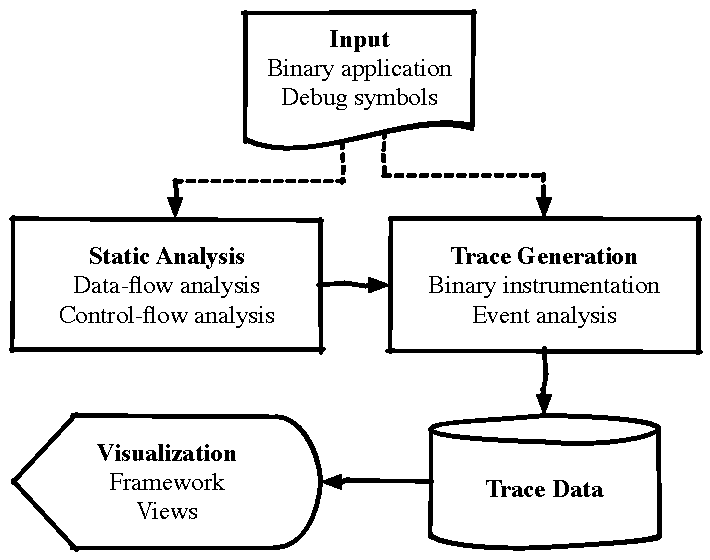
\includegraphics[width=0.40\textwidth]{img/parceive}
		\caption{The high-level components of Parceive.}
		\label{fig:parceive_overview}
	\end{center}
\end{figure}

Figure \ref{fig:parceive_overview} depicts the fundamental components of
Parceive and their relations. Our analyses operate on executables to retrieve
the required information. These analyses can be classified into static and
dynamic ones. The former inspect the data- and control-flow of single linkage
objects. By incorporating debug symbols, static analysis enables our tool to
gather information about variable accesses, loop constructs, and class
hierarchies. Additionally, the gathered information is used to restrict the
scope of subsequent runtime analysis in order to reduce the execution overhead.

The runtime analysis instruments and inspects predefined events during
execution of an application, e.g., object instantiations, method invocations,
and thread handling (in case of multi-threaded applications). During such
events, Parceive collects trace data and stores it in an SQL database. The
database scheme enables highly specific and performant queries for different
visualizations which are key for program comprehension and parallelization.
Each view thereby simplifies and highlights specific aspects of the traced
software.